%%%%%%%%%%%%%%%%%%%%%%% file template.tex %%%%%%%%%%%%%%%%%%%%%%%%%
%
% This is a general template file for the LaTeX package SVJour3
% for Springer journals.          Springer Heidelberg 2010/09/16
%
% Copy it to a new file with a new name and use it as the basis
% for your article. Delete % signs as needed.
%
% This template includes a few options for different layouts and
% content for various journals. Please consult a previous issue of
% your journal as needed.
%
%%%%%%%%%%%%%%%%%%%%%%%%%%%%%%%%%%%%%%%%%%%%%%%%%%%%%%%%%%%%%%%%%%%
%
% First comes an example EPS file -- just ignore it and
% proceed on the \documentclass line
% your LaTeX will extract the file if required
\begin{filecontents*}{example.eps}
%!PS-Adobe-3.0 EPSF-3.0
%%BoundingBox: 19 19 221 221
%%CreationDate: Mon Sep 29 1997
%%Creator: programmed by hand (JK)
%%EndComments
gsave
newpath
  20 20 moveto
  20 220 lineto
  220 220 lineto
  220 20 lineto
closepath
2 setlinewidth
gsave
  .4 setgray fill
grestore
stroke
grestore
\end{filecontents*}
%
\RequirePackage{fix-cm}
%
%\documentclass{svjour3}                     % onecolumn (standard format)
%\documentclass[smallcondensed]{svjour3}     % onecolumn (ditto)
%\documentclass[smallextended]{svjour3}       % onecolumn (second format)
\documentclass[twocolumn]{svjour3}          % twocolumn
%
\smartqed  % flush right qed marks, e.g. at end of proof
\usepackage{graphicx}
\usepackage{float}


\begin{document}
\begin{figure}[H]
  \centering
    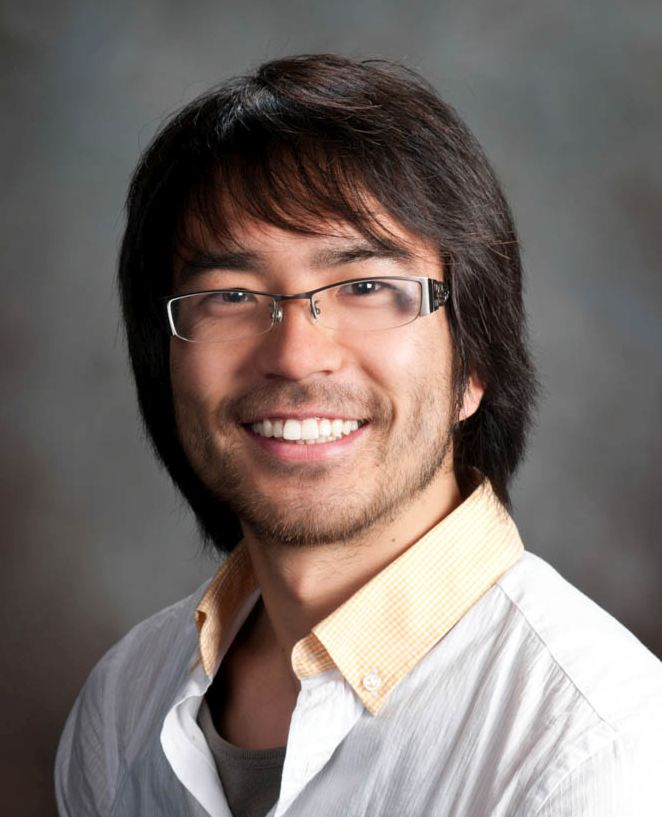
\includegraphics[width=1in,clip,keepaspectratio]{takami.jpg}
\end{figure}
\noindent\textbf{Kuya Takami} is pursuing his Ph.D. in Mechanical Engineering at Virginia Polytechnic Institute and State University (Virginia Tech), USA. He previously earned his B.S. and M.S. at University of Wisconsin-Madison in 2008, and 2011. He works under Computational Multi-physics and Systems Laboratory, and National Science Foundation funded Center for Tire Research. His primary interests expands in acoustic, and experimental/ computational mechanics and robotics fields. He has worked on autonomous driving based on simultaneous localization and mapping, and currently working on non-field-of-view acoustic target localization and noise prediction of the automotive tires.
\begin{figure}[H]
  \centering
 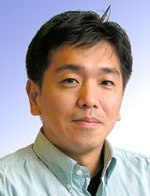
\includegraphics[width=1in,clip,keepaspectratio]{furukawa.jpg}
\end{figure}
\noindent\textbf{Tomonari Furukawa} is a professor at Virginia Tech and Directors of Computational Multiphysics Systems Lab. He received the B.Eng. in Mechanical Engineering from Waseda University, Japan, in 1990, the M.Eng. in Mechatronic Engineering from University of Sydney, Australia, in 1993 and Ph.D in Quantum Engineering and Systems Science from University of Tokyo, Japan, in 1996.  He worked at the University of Tokyo, the University of Sydney, and the University of New South Wales as faculty. His research work focuses on inverse analysis and optimization methods in experimental/ computational mechanics and robotics.  He has published over 250 technical papers and won various early career research awards and paper awards including the most prestigious computational mechanics young investigator award from International Association for Computational Mechanics.  He has also led several international competitions and is currently leading Virginia Tech’s Team VALOR for DARPA Robotics Challenge, which is one of the 11 finalists for the challenge. 
\begin{figure}[H]
  \centering
    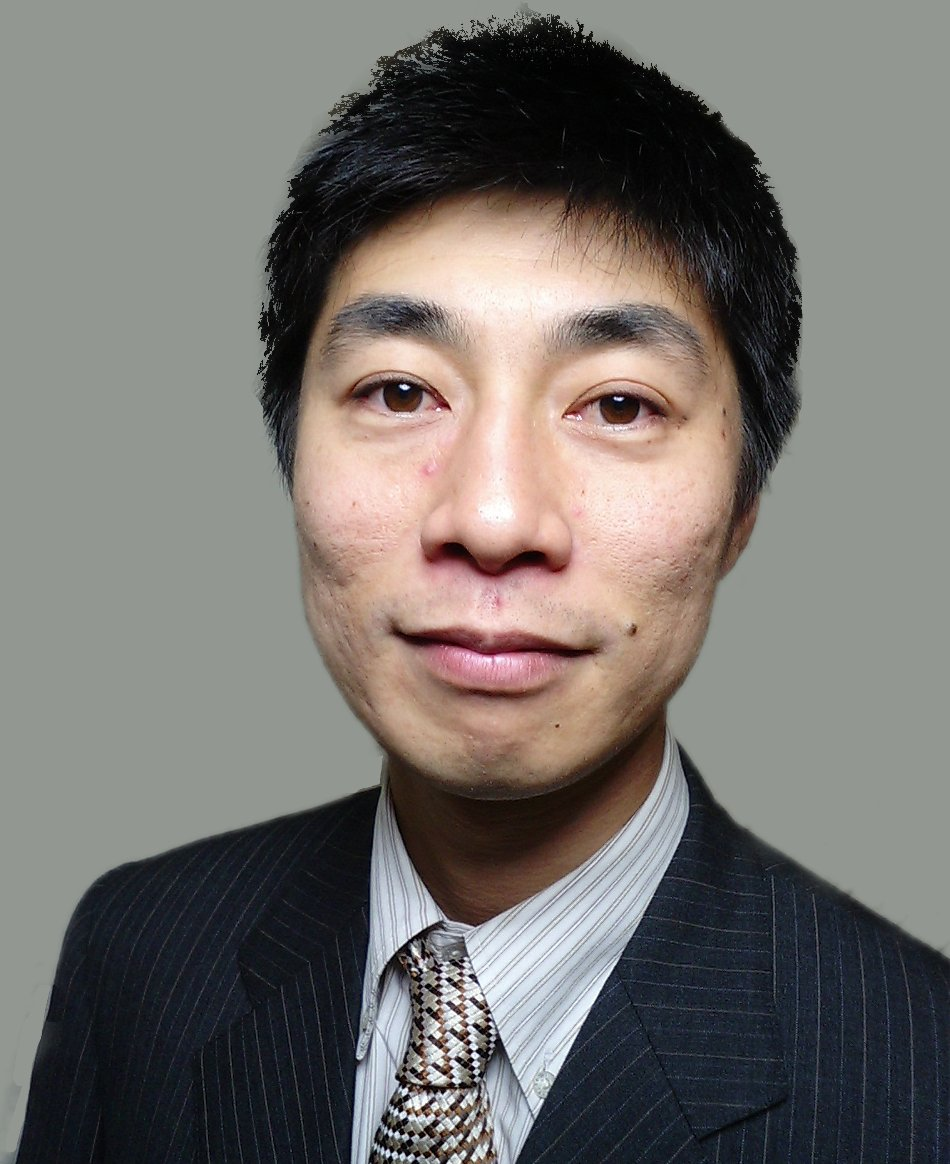
\includegraphics[width=1in,clip,keepaspectratio]{kumon.jpg}
\end{figure}
\noindent\textbf{Makoto Kumon} received the B.S. in applied mathematics and physics, the M.S. in applied systems science, and the Ph.D. degree in Informatics all from Kyoto University, Kyoto, Japan, in 1994, 1996 and 2002 respectively. From 2000 to 2005, he was a Research Associate in the Department of Mechanical Engineering and Materials Science at the Kumamoto University, Kumamoto, Japan, where he is currently working as an Associate Professor of Department of Intelligent Mechanical Systems. His research interest includes path-following control of robots, auditory robots and UAV systems. Dr. Kumon is a member of IEEE, ASME, AIAA and RSJ. 
\begin{figure}[H]
  \centering
 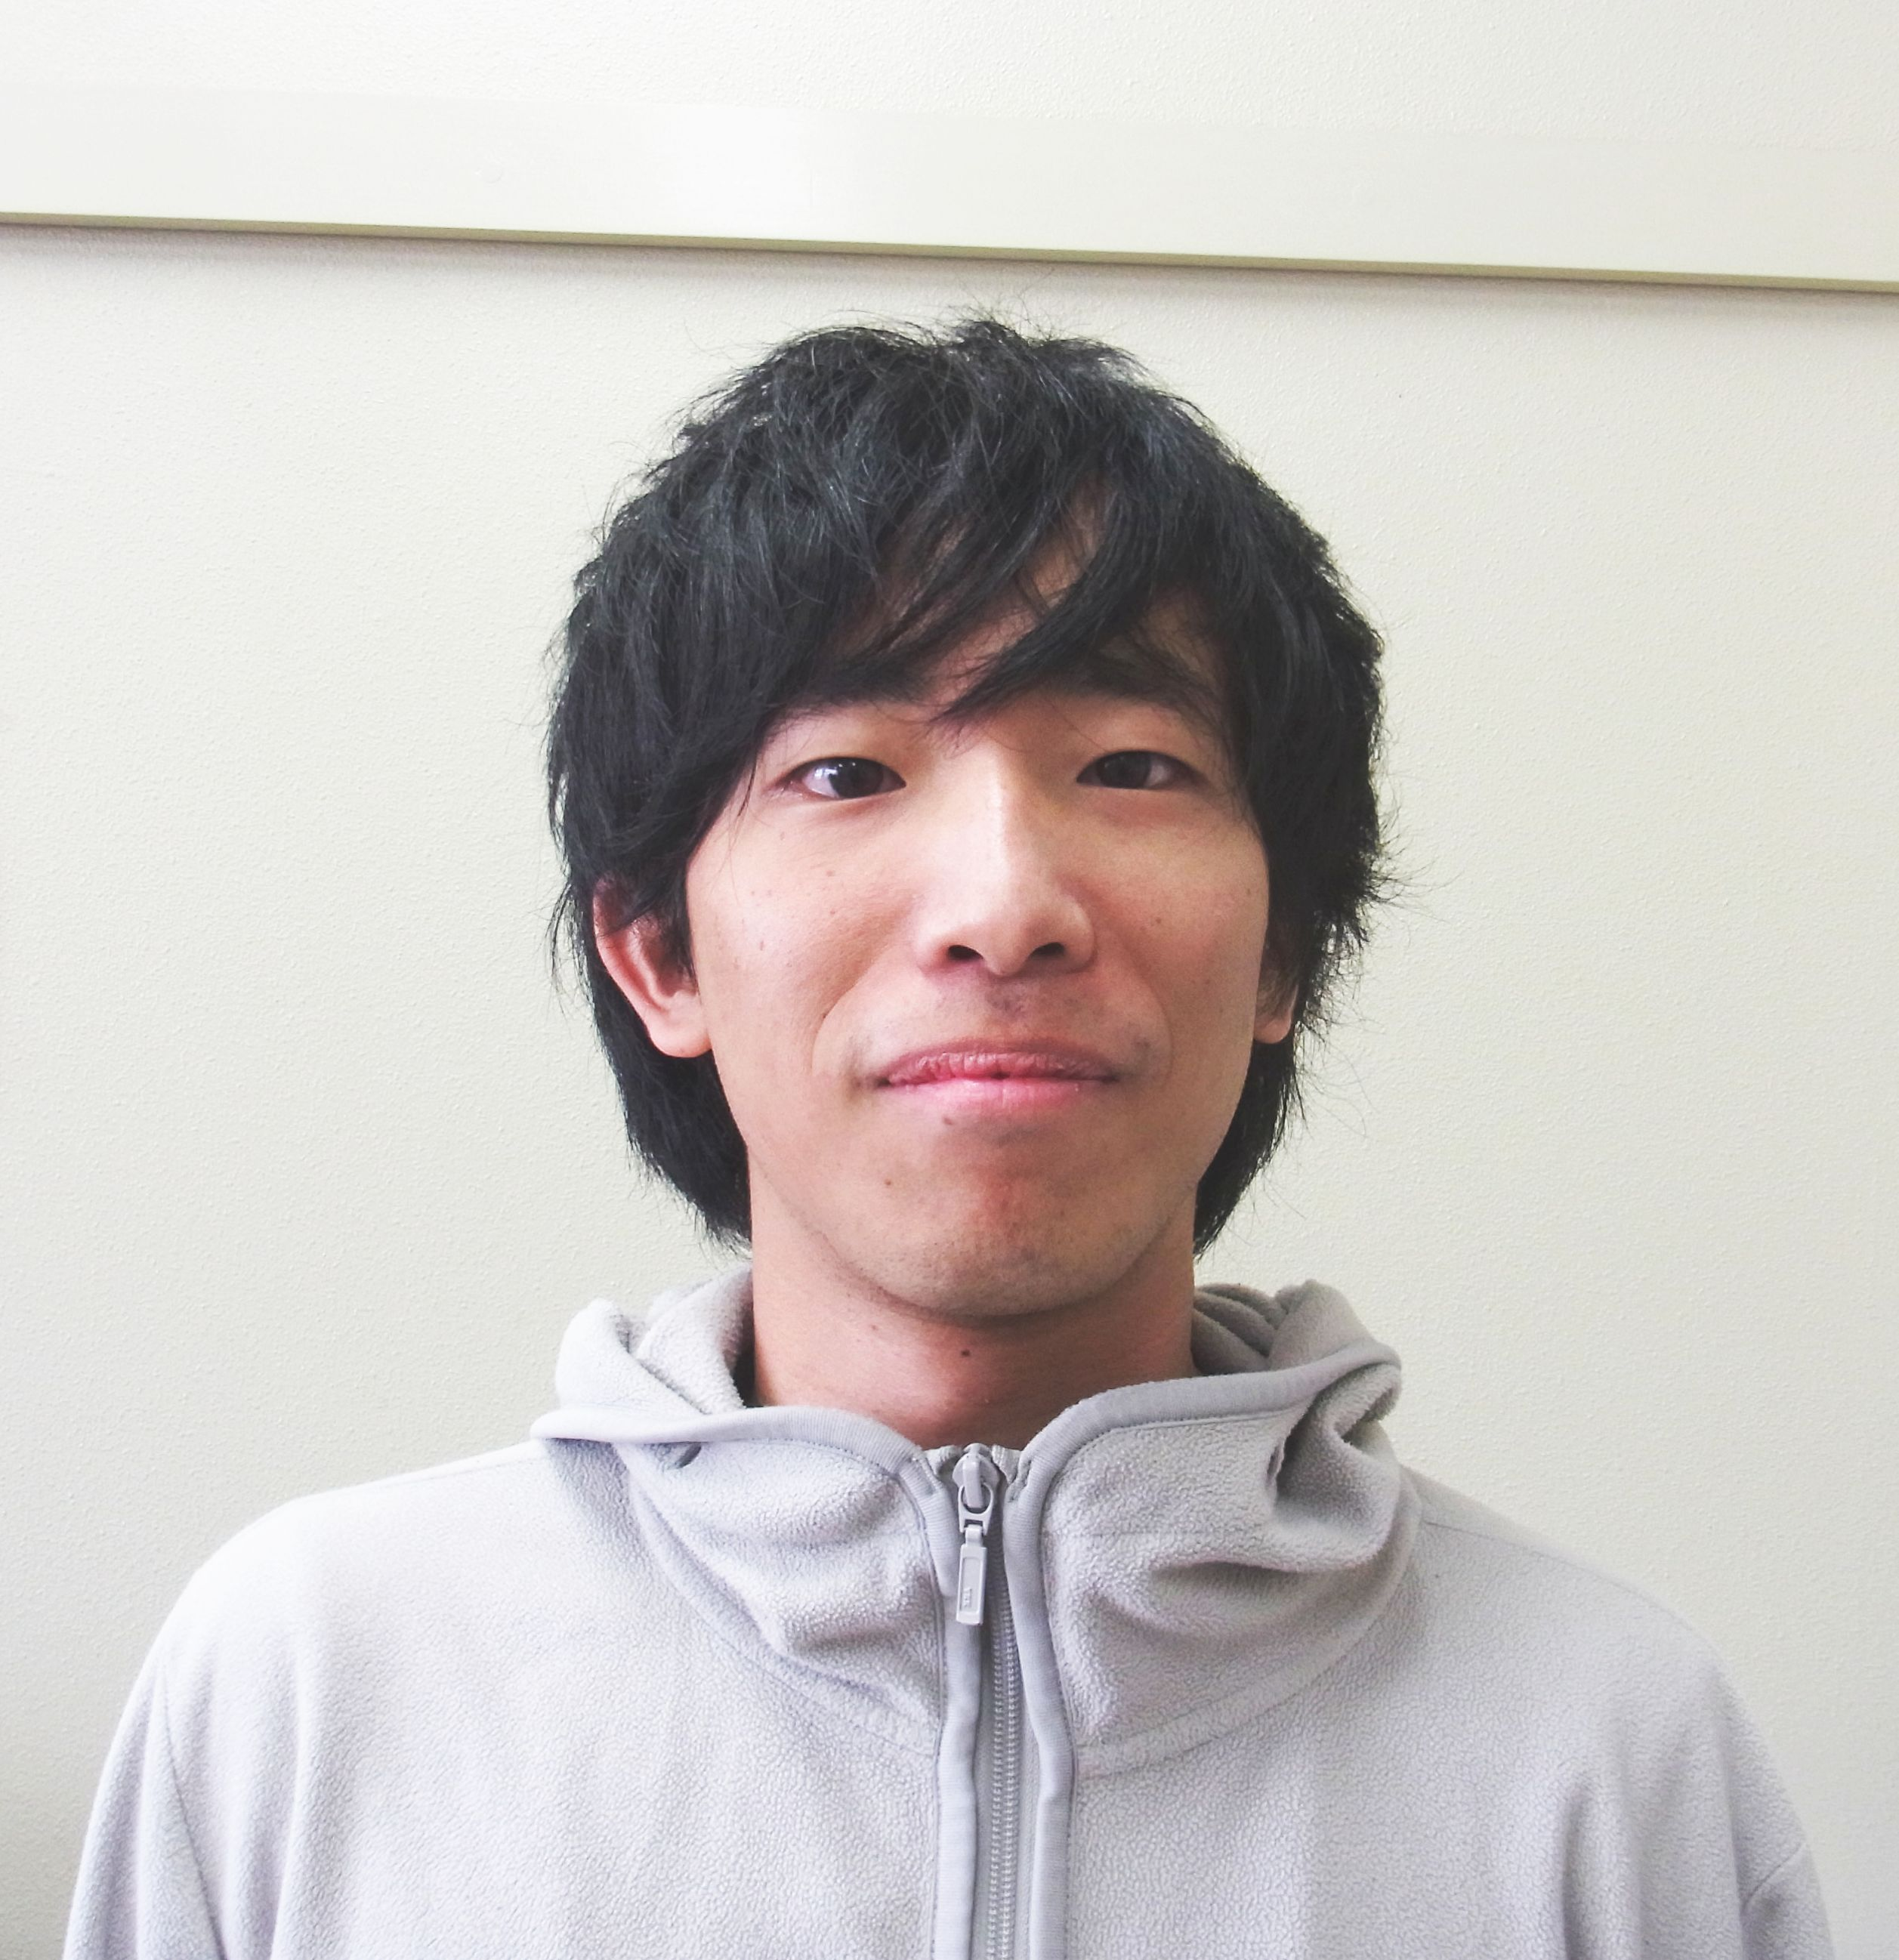
\includegraphics[width=1in,clip,keepaspectratio]{kimoto.jpg}
\end{figure}
\noindent\textbf{Daisuke Kimoto} received the B.S. and the M.S. in Mechanical Engineering from Kumamoto University in 2012 and 2014 respectively. He has been with Daihatsu Motor Kyushu Co. since 2014. His research interests includes binaural robot audition and probablistic sound source localization.
\begin{figure}[H]
  \centering
 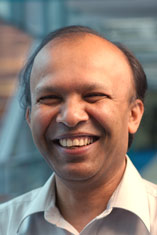
\includegraphics[width=1in,clip,keepaspectratio]{dissanayake.jpg}
\end{figure}
\noindent\textbf{Gamini Dissanayake} is the James N Kirby Professor of Mechanical and Mechatronic Engineering at University of Technology, Sydney (UTS). He has expertise in a broad range of topics in robotics including sensor fusion, localisation, mapping, SLAM and human-robot interaction. He leads the UTS node of the Australian Research Council Centre of Excellence for Autonomous Systems (CAS), UTS Centre for Intelligent Mechatronic Systems (CIMS) and the UTS robotics team. He graduated in Mechanical/Production Engineering from the University of Peradeniya, Sri Lanka in 1977. He received his M.Sc. in Machine Tool Technology and Ph.D. in Mechanical Engineering (Robotics) from the University of Birmingham, England in 1981 and 1985 respectively.

 
\end{document}

